\documentclass[a4paper,10pt]{article}
\usepackage[utf8]{inputenc}
\usepackage[english,russian]{babel}
\usepackage{fancyhdr}
\usepackage{caption}

\usepackage{listings,longtable,amsmath,amsfonts,graphicx,tikz,tabularx}
\usetikzlibrary{automata}
\usepackage{algpseudocode}

\captionsetup{labelsep=period}
\pagestyle{fancy}

\lstset{
    basicstyle=\footnotesize,
    breakatwhitespace=false,
    breaklines=true,
    extendedchars=true,
    keepspaces=true,
    keywordstyle=\bfseries,
    numbers=left,
    numbersep=3pt,
    numberstyle=\tiny,
    showspaces=false,
    showstringspaces=false,
    showtabs=false,
    stepnumber=1,
    stringstyle=\emph,
    tabsize=2
}


\tikzset{
    min/.style = {circle, draw=gray,fill=gray, text=white, thick}
}

\usepackage[left=1.5cm,right=1.5cm,top=2cm,bottom=1.5cm,bindingoffset=0cm]{geometry}

\captionsetup{labelsep=period}
\pagestyle{fancy}

\renewcommand{\headrulewidth}{0pt}
\fancyfoot[L] {\thepage\bf}
\fancyfoot[C] {}

\graphicspath{ {img/} }

\begin{document}
    \begin{titlepage}
        \begin{center}
            \large
            САНКТ-ПЕТЕРБУРГСКИЙ НАЦИОНАЛЬНЫЙ ИССЛЕДОВАТЕЛЬСКИЙ УНИВЕРСИТЕТ ИНФОРМАЦИОННЫХ ТЕХНОЛОГИЙ, МЕХАНИКИ И ОПТИКИ \\


            \vspace{3cm}


            Кафедра вычислительной техники
            \vspace{4cm}

            \textsc{ \textbf{Отчёт по лабораторной работе  № 1} \\
            по дисциплине <<Тестирование программного обеспечения>>\\}
            Вариант №776\\[8mm]

            \bigskip
        \end{center}
        \vspace{3cm}

        \hfill\begin{flushright}
             Студенты: \\ Куклина М. \\ Кириллова А. 
             \vfill
             Преподаватель: \\ Клименков C.В. 
        \end{flushright}
        \vfill
        \vfill
        \vfill
        \vfill
        \vfill
        \begin{center}
            Санкт-Петербург \\2017 г.
        \end{center}
    \end{titlepage}
\newpage
\section*{Задание}
\begin{enumerate}
    \item  Для указанной функции провести модульное тестирование разложения функции в степенной ряд. Выбрать достаточное тестовое покрытие. \\
        \textit{Функция sec().}
    \item  Провести модульное тестирование указанного алгоритма. Для этого выбрать характерные точки внутри алгоритма, и для предложенных самостоятельно наборов исходных данных записать последовательность попадания в характерные точки. Сравнить последовательность попадания с эталонной. \\
        \textit{Программный модуль для работы с Фибоначчиевой кучей }
    \item Сформировать доменную модель для заданного текста.  Разработать тестовое покрытие для данной доменной модели \\
        \textit{В первый момент показалось, что ничего не произошло, затем что-то засветилось на краю огромного экрана. 
        По нему ползла красная звезда величиной с тарелку, а следом за ней еще одна: бинарная звездная система.
        Затем в углу картинки возник большой полумесяц -- красный свет, переходящий в черноту -- ночная сторона планеты. }
\end{enumerate}
\section*{Тестирование функции sec()}
Для создания тестового покрытия были выделены классы эквивалентности, то есть промежутки, где функция меняется одинаково:
\begin{enumerate}
    \item $(\frac {-3\pi} {2} + 2\pi n; \frac {-\pi} {2} + 2\pi n), n \in Z$
    \item $(\frac {-\pi} {2} + 2\pi n; \frac {\pi} {2} + 2\pi n), n \in Z$
    \item Точки, в которых функция неопределена: $\frac {\pi} {2} + \pi n, n \in Z$.

\begin{figure}[h!]
	\caption{График функции}
	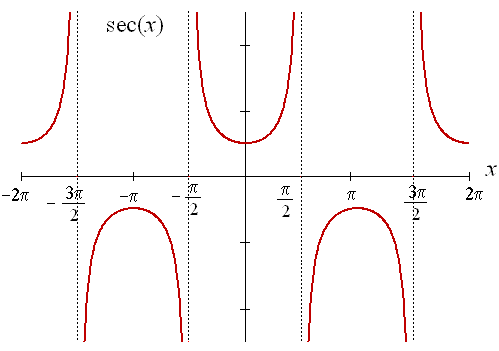
\includegraphics[scale=0.4]{./img/sec_plot.png}
\end{figure}

\end{enumerate}

\section*{Тестирование модуля Fibonacci Heap}

    \subsection*{Функции модуля}
        \subsubsection*{Вставкa}
            \begin{algorithmic}[1]
                \Function {$Fib\_Heap\_Insert$} {$H, x$}
                    \State $degree[x] \gets 0 $
                    \State $p[x] \gets NIL$
                    \State $child[x] \gets NIL$
                    \State $left[x] \gets x$
                    \State $right[x] \gets x$
                    \State $mark[x] \gets falsa$
                    \State \text{Merge roots list of x and H}
                    \If {\text{$min[H] = Nil$ or $key[x] < key[min[H]]$}}
                        \State $min[H] \gets x$
                    \EndIf
                    \State $n[H] \gets n[H] + 1$
                \EndFunction      
            \end{algorithmic}

        \begin{figure}[h!]
            \caption{Вставка элемента 1}
            \label{fig:insert_fst_step}
            \center
            \begin{tikzpicture}[auto,node distance=2cm, semithick]
                \tikzstyle{every state}=[draw=black,text=black,fill=white,thick]
                \node[min] (A1)   {$1$};
            \end{tikzpicture}
        \end{figure}

        \begin{figure}[h!]
            \caption{Вставка элемента 2}
            \label{fig:insert_snd_step}
            \center
            \begin{tikzpicture}[auto,node distance=2cm, semithick]
                \tikzstyle{every state}=[draw=black,text=black,fill=white,thick]
                \node[min] (A1)               {$1$};
                \node[state] (A2)[left of=A1]   {$2$};
                
                \path (A1) edge node {$ $}(A2)
                      (A2) edge node {$ $}(A1);
            \end{tikzpicture}
        \end{figure}

        \begin{figure}[h!]
            \caption{Вставка элемента 3}
            \label{fig:insert_thd_step}
            \center
            \begin{tikzpicture}[auto,node distance=2cm, semithick]
                \tikzstyle{every state}=[draw=black,text=black,fill=white,thick]
                \node[min] (A1)               {$1$};
                \node[state] (A2)[left of=A1]   {$2$};
                \node[state] (A3)[left of=A2]   {$3$};
                \path (A1) edge node {$ $}(A2)
                      (A2) edge node {$ $}(A3)
                      (A3) edge[bend right] node {$ $}(A1);
            \end{tikzpicture}
        \end{figure}

        \begin{figure}[h!]
            \caption{Вставка элемента 0}
            \label{fig:insert_fth_step}
            \center
            \begin{tikzpicture}[auto,node distance=2cm, semithick]
                \tikzstyle{every state}=[draw=black,text=black,fill=white,thick]
                \node[min] (A1)               {$1$};
                \node[state] (A0)[left of=A1]   {$1$};
                \node[state] (A2)[left of=A0]   {$2$};
                \node[state] (A3)[left of=A2]   {$3$};
                
                \path (A1) edge node {$ $}(A0)
                      (A0) edge node {$ $}(A2)
                      (A2) edge node {$ $}(A3)
                      (A3) edge[bend right] node {$ $}(A1) ;
            \end{tikzpicture}
        \end{figure}
        \begin{table}[h!]
            \begin{tabular}{|c|c|c|c|}
                \hline
                Шаг & Ключ & min   & Рисунок                        \\ \hline
                0    & x   &  null & Initialize heap.               \\ \hline
                1    & 1   &  1    & Рис.~\ref{fig:insert_fst_step} \\ \hline
                2    & 2   &  1    & Рис.~\ref{fig:insert_snd_step} \\ \hline
                3    & 3   &  1    & Рис.~\ref{fig:insert_thd_step} \\ \hline
                4    & 0   &  0    & Рис.~\ref{fig:insert_fth_step} \\ \hline
            \end{tabular}
            \caption{Эталонная таблица вставок.}
			\center
        \end{table}

        \subsubsection*{Минимальный узел}
            \begin{algorithmic}[1]
                \Function {$Fin\_Minimum$}{$ $}
                    \State \Return $min$
                \EndFunction
            \end{algorithmic}

        \subsubsection*{Объединение двух куч}
            \begin{algorithmic}[1]
                \Function {$Fib\_Heap\_Union$} {$H_1$, $H_2$}
                    \State $H \gets Make\_Fib\_Heap()$
                    \State $min[H] \gets min[H_1]$
                    \State \text{Add roots of $H_2$ to H.}
                    \If {\text{$min[H_1] = NIL$ or $min[H_2] \ne NIL$ and $key[min[H_2]] < key[min[H_1]]$}}
                        \State $min[H] \gets min[H_2]$
                    \EndIf
                    \State $n[H] \gets n[H_1] + n[H_2]$
                    \State \Return $H$
                \EndFunction
            \end{algorithmic}

        \begin{figure}[h!]
            \caption{Этап 1: Куча.}
            \label{fig:merge_step_1}
            \center
            \begin{tikzpicture}
                \node[min] (a) {$6$}
                        child {node[circle,draw] (b) {$2$}}
                        child {node[circle,draw] (c) {$3$}
                            child {node[circle,draw] (d) {$4$}}
                        };
            \end{tikzpicture}
        \end{figure}

        \begin{figure}[h!]
            \caption{Этап 2: Добавление корней в список H.}
            \label{fig:merge_step_2}
            \center
            \begin{tikzpicture}[auto,node distance=2cm, semithick]
                \node[min] (a) {$1$};
            \end{tikzpicture}
        \end{figure}

        \begin{figure}[h!]
            \caption{Этап 3: Итоговая куча.}
            \label{fig:merge_step_3}
            \center
            \begin{tikzpicture}[auto,node distance=2cm, semithick]
                \node[min] (a) {$1$}
                        child {node[circle,draw] (b) {$2$}}
                        child {node[circle,draw] (c) {$3$}
                            child {node[circle,draw] (d) {$4$}}
                        };
            \end{tikzpicture}
        \end{figure}

        \begin{table}[h!]
            \caption{Последовательность объединенaя пустой кучи и кучи}
			\center
            \begin{tabular}{|c|c|c|c|}
                \hline
                Шаг  & Линия &  Рисунок                     & Комментарий                 \\ \hline
                  1  &   x   &  Рис.~\ref{fig:merge_step_1} & Даём функции два дерева; допустим, $H_1$ пустое.    \\ \hline
                  2  &   4   &  Рис.~\ref{fig:merge_step_2} & Добавляем корни $H_2$ в $H$. \\ \hline
                  3  &  5-9  &  Рис.~\ref{fig:merge_step_3} & Так как $min[H_1] = NIL$, обновляем $min[H]$; возвращаем кучу. \\ \hline
            \end{tabular}
        \end{table}

        \begin{figure}[h!]
            \caption{Этап 1: Две кучи}
            \label{fig:merge_step_11}
            \center
            \begin{tikzpicture}[auto, semithick]
                \node[min] (a) {$1$}
                    child {node[circle,draw] (b) {$2$}}
                    child {node[circle,draw] (c) {$3$}
                        child {node[circle,draw] (d) {$4$}}
                    };
            \end{tikzpicture}
            \begin{tikzpicture}[auto, semithick]
                    \node[circle,draw] (a) {$6$}
                        child {node[circle,draw] (b) {$7$}}
                        child {node[circle,draw] (c) {$8$}
                            child {node[circle,draw] (d) {$9$}}
                        };
            \end{tikzpicture}
        \end{figure}

        \begin{figure}[h!]
            \caption{Этап 2: Добавление корней $H_2$ в $H$}
            \label{fig:merge_step_21}
            \center
            \begin{tikzpicture}[auto, semithick]
                    \node[circle,draw] (a) {$6$};
            \end{tikzpicture}
        \end{figure}

        \begin{figure}[h!]
            \caption{Этап 3: Результатирующая куча}
            \label{fig:merge_step_31}
            \center
            \begin{tikzpicture}[auto, semithick, node distance=3cm]
                \node[min] (a) {$1$}
                    child {node[circle,draw] (b) {$2$}}
                    child {node[circle,draw] (c) {$3$}
                        child {node[circle,draw] (d) {$4$}}
                    };
                \node[circle,draw] (a1)[left of=a] {$6$}
                    child {node[circle,draw] (b1) {$7$}}
                    child {node[circle,draw] (c1) {$8$}
                        child {node[circle,draw] (d1) {$9$}}
                    };
                \path (a) edge node{$ $} (a1);
            \end{tikzpicture}
        \end{figure}

        \begin{table}[h!]
            \caption{Последовательность объединения двух куч}
			\center
            \begin{tabular}{|c|c|c|c|}
                \hline
                Шаг  & Линия &  Рисунок                      & Комментарий                \\ \hline
                  1  &   x   &  Рис.~\ref{fig:merge_step_11} & Даём функции два дерева.    \\ \hline
                  2  &   4   &  Рис.~\ref{fig:merge_step_21} & Добавляем корни $H_2$ в $H$. \\ \hline
                  3  &  5-9  &  Рис.~\ref{fig:merge_step_31} & Возвращаем кучу. \\ \hline
            \end{tabular}
        \end{table}

        \subsubsection*{Извлечение минимального узла}

            \begin{algorithmic}[1]
                \Function{$Fib\_Heap\_Extract\_Min$}{$ $}
                    \State $z \gets min[H]$
                    \If {$z \ne NIL$}
                        \For {\text{Each child x of z}}
                            \State \text{Add x to roots list.}
                            \State $p[x] \gets NIL$
                        \EndFor
                        \State \text{Remove z from roots list.}
                        \If {$z = right[z]$}
                            \State $min[H] \gets NIL$
                        \Else
                            \State $min[H] \gets right[z]$
                            \State $Consolidate(H)$
                        \EndIf
                    \EndIf
                    \State $n[H] \gets n[H] - 1$
                \EndFunction
            \end{algorithmic}
            \begin{algorithmic}[1]
                \Function{$Consolidate$}{$ $}
                    \For {\text{$i \gets 0$ to $D(n[H])$}}
                        \State $A[i] \gets NIL$
                    \EndFor
                    \For {\text{Each w in roots list of H}}
                        \State $x \gets w$
                        \State $d \gets degree[x]$
                        \While {$A[d] \neq NIL$}
                            \State $y \gets A[d]$
                            \If {$key[x] > key[y]$}
                                \State $swap(x,y)$
                            \EndIf
                            \State $Fib\_Heap\_Link(H, y, x)$
                            \State $A[d] \gets NIL$
                            \State $d \gets d + 1$
                        \EndWhile
                        \State $A[d] \gets x$
                    \EndFor
                    \State $min[H] \gets NIL$
                    \For \text{$i \gets 0$ to $D(n[H])$}
                        \If {$A[i] \neq NIL$}
                            \State \text{Add A[i] to roots list of H}
                            \If {\text{$min[H] = NIL$ or $key[A[i]] < key[min[H]]$}}
                                \State $min[H] \gets A[i]$
                            \EndIf
                        \EndIf
                    \EndFor
                \EndFunction
            \end{algorithmic}
            \begin{algorithmic}[1]
                \Function{$Fib\_Heap\_Link$}{$H, y, x$}
                    \State \text{Remove y from roots list of H}
                    \State \text{Merge y and child[x] list}
                    \State $degree[x] \gets degree[x] + 1$
                    \State $mark[y] \gets false$
                \EndFunction
            \end{algorithmic}
 

            \begin{figure}[h!]
                \caption{Начальная куча}
                \label{fig:extract_one_step_1}
                \center
                \begin{tikzpicture}
                    \node[min] (a) {$1$};
                \end{tikzpicture}
            \end{figure} 
            \begin{table}[h!]
                \caption{Последовательность извлечение минимального узла}
    			\center
                \begin{tabular}{|c|c|c|c|}
                    \hline
                    Шаг  & Линия &  Рисунок                           & Комментарий                \\ \hline
                      1  & 2-3   &  Рис.~\ref{fig:extract_one_step_1} & Минимальное значение не равно $NIL$ \\ 
                      2  & 4     &                                 & поэтому просматриваем детей, одно их нет. \\
                      3  & 8     &                                 & Затем удаляем элемент из списка корней. \\ 
                      4  & 9     &                                 & Так как элемент был один, то его правый указатель указывает на него же. \\
                      5  & 10    &                                 & Поэтому минимальный элемент обращается в $NIL$. \\ \hline
                \end{tabular}
            \end{table}


            \begin{figure}[h!]
                \caption{Начальная куча}
                \label{fig:extract_step_1}
                \center
                \begin{tikzpicture}[auto, semithick, node distance=3cm]
                \node[min] (a) {$1$}
                    child {node[circle,draw] (b) {$2$}
                        child {node[circle,draw] (d) {$5$}}
					}
                    child {node[circle,draw] (c) {$3$}
                        child {node[circle,draw] (d) {$4$}}
                    };
                \node[circle,draw] (a1)[left of=a] {$6$}
                    child {node[circle,draw] (b1) {$7$}}
                    child {node[circle,draw] (c1) {$8$}
                        child {node[circle,draw] (d1) {$9$}}
                    };
                \path (a) edge node{$ $} (a1);
                \end{tikzpicture}
            \end{figure} 

            \begin{figure}[h!]
                \caption{Записываем детей в список корней.}
                \label{fig:extract_step_2}
                \center
                \begin{tikzpicture}[auto, semithick, node distance=3cm]
                    \node[circle,draw] (b) {$2$}
                        child {node[circle,draw] (d) {$5$}} ;
                    \node[circle,draw] (c)[left of = b] {$3$}
                        child {node[circle,draw] (d) {$4$}};
                    \node[circle,draw] (a1)[left of=c] {$6$}
                        child {node[circle,draw] (b1) {$7$}}
                        child {node[circle,draw] (c1) {$8$}
                            child {node[circle,draw] (d1) {$9$}}
                        };
                \path (b) edge node{$ $} (c)
                      (c) edge node{$ $} (a1)
                      (a1) edge[bend left] node{$ $} (b);
                \end{tikzpicture}
            \end{figure} 

            \begin{figure}[h!]
                \caption{Добавляем ноду 3 в список детей ноды 2}
                \label{fig:extract_step_3}
                \center
                \begin{tikzpicture}[auto, semithick, node distance=3cm]
                    \node[circle,draw] (b) {$2$}
                        child {node[circle,draw] (d) {$5$}} 
                        child {node[circle,draw] (c) {$3$}
                        	child {node[circle,draw] (d) {$4$}}
						};
                    \node[circle,draw] (a1)[left of=b] {$6$}
                        child {node[circle,draw] (b1) {$7$}}
                        child {node[circle,draw] (c1) {$8$}
                            child {node[circle,draw] (d1) {$9$}}
                        };
                \end{tikzpicture}
            \end{figure} 
            \begin{figure}[h!]
                \caption{Добавляем ноду 6 в список детей ноды 2}
                \label{fig:extract_step_4}
                \center
                \begin{tikzpicture}[auto, semithick, node distance=3cm]
                    \node[circle,draw] (b) {$2$}
                        child { node[circle,draw] (d) {$5$}} 
                        child { node[circle,draw] (c) {$3$}
                        	child {node[circle,draw] (d) {$4$}}
						}
                        child {node[circle,draw] (a1) {$6$}
                            child {node[circle,draw] (b1) {$7$}}
                            child {node[circle,draw] (c1) {$8$}
                                child {node[circle,draw] (d1) {$9$}}
							}
                        };
                \end{tikzpicture}
            \end{figure} 
            \begin{table}[h!]
                \caption{Последовательность извлечение минимального узла}
    			\center
                \begin{tabular}{|c|c|c|c|}
                    \hline
                    Шаг  & Линия &  Рисунок                       & Комментарий                \\ \hline
                      1  & 2-3   &  Рис.~\ref{fig:extract_step_1} & Минимальное значение не равно $NIL$ \\ 
                      2  & 4-7   &  Рис.~\ref{fig:extract_step_2} & Записываем детей минимальной ноды в список корней $H$ \\
    				  3  & 9-14  &								  & Правый указатель указывает не на себя же, поэтому меняем $min$ \\
    					 &       &								  & и запускаем функцию $Consolidate(H)$  \\ \hline
    				  4  &  5-18 &	Рис.~\ref{fig:extract_step_3} & Для нод с одинаковым уровнем делаем большую ноду ребёнком меньшей. \\ \hline
    				  5  &  5-18 &	Рис.~\ref{fig:extract_step_4} & Для нод с одинаковым уровнем делаем большую ноду ребёнком меньшей. \\ \hline
					  6  &  20-27&  Рис.~\ref{fig:extract_step_4} & Так как нода одна не происходит объединения. \\ \hline
                \end{tabular}
            \end{table}
        \newpage
        \newpage
        \subsubsection*{Уменьшение ключа}
            \begin{algorithmic}[1]
                \Function {$Finc\_Heap\_Decrease\_Key$} {$H, x, k$}
                    \If {$k > key[x]$}
                        \State \textbf{error} \text{New key is bigger than old one.}
                    \EndIf
                    \State $key[x] \gets k$
                    \State $y \gets p[x]$
                    \If {\text{$y \neq NIL$ and $key[x] < key[y]$}}
                        \State $Cut(H, x, y)$
                        \State $Cascading\_Cut(H, y)$
                    \EndIf
                    \If {$key[x] < key[min[H]]$}
                        \State $min[H] \gets x$
                    \EndIf
                \EndFunction
            \end{algorithmic}

            \begin{algorithmic}[1]
                \Function{$Cut$} {$H, x, y$}
                    \State \text{Delete x from child list of y}
                    \State $degree[y] \gets degree[y] - 1$
                    \State \text{Add x to roots list H}
                    \State $p[x] \gets NIL$
                    \State $mark[x] \gets false$
                \EndFunction
            \end{algorithmic}
            \begin{algorithmic}[1]
                \Function{$Cascading\_Cut$}{$H, y$}
                    \State $z \gets p[y]$
                    \If {$z \neq NIL$}
                        \If {$mark[y] = true$}
                            \State $mark[y] = false$
                        \Else
                            \State $Cut(H, y, z)$
                            \State $Cascading\_Cut(H, z)$
                        \EndIf
                    \EndIf
                \EndFunction 
            \end{algorithmic}
            \begin{figure}[h!]
                \caption{Начальная куча}
                \label{fig:dec_one_step_1}
                \center
                \begin{tikzpicture}[auto, semithick, node distance=3cm]
                    \node[min] (a) {$1$}
						child{ node[circle,draw] (b) {$2$}};
                \end{tikzpicture}
            \end{figure} 
            \begin{figure}[h!]
                \caption{В функции $Cut()$}
                \label{fig:dec_one_step_2}
                \center
                \begin{tikzpicture}[auto, semithick, node distance=3cm]
                    \node[min] (a) {$1$};
				    \node[circle,draw] (b)[left of=a] {$0$};
					\path (a) edge node{$ $} (b)
					      (b) edge[bend right] node{$ $} (a);
                \end{tikzpicture}
            \end{figure} 
            \begin{figure}[h!]
                \caption{Итоговая куча}
                \label{fig:dec_one_step_3}
                \center
                \begin{tikzpicture}[auto, semithick, node distance=3cm]
                    \node[circle,draw] (a) {$1$};
				    \node[min] (b)[left of=a] {$0$};
					\path (a) edge node{$ $} (b)
					      (b) edge[bend right] node{$ $} (a);
                \end{tikzpicture}
            \end{figure} 
            \begin{table}[h!]
                \caption{Последовательность изменения минимального узла}
    			\center
                \begin{tabular}{|c|c|c|c|}
                    \hline
                    Шаг  & Линия &  Рисунок                       & Комментарий                \\ \hline
					1    &   5   & Рис.~\ref{fig:dec_one_step_1}  & Уменьшим ноду 2 до 0.\\ \hline
					2    &   5-6 &								  & Именяем ключ; записываем в y ноду 1. \\ \hline
					3    &  7    &							      & Заходим в тело \textbf{if}. \\ \hline
					4    &  8    & Рис.~\ref{fig:dec_one_step_2}  & Заходим в функцию $Cut()$ \\ \hline
					5    &  9    & 								  & Выходим из функции $Cascading\_Cut()$ без изменений. \\ \hline
					6    &  12   & Рис.~\ref{fig:dec_one_step_3}  & Так как $0 < 1$ меняем минимальный ключ. \\ \hline 
                \end{tabular}
            \end{table}


        \subsubsection*{Удаление элемента}
            \begin{algorithmic}[1]
                \Function{$Fib\_Heap\_Delete$}{$ $}
                    \State $Fib\_Heap\_Decrease\_Key(H, x,-\infty)$
                    \State $Fib\_Heap\_Extract\_Min(H, x)$
                \EndFunction
            \end{algorithmic}
            \begin{table}[h!]
                \caption{Последовательность удаления узла}
    			\center
                \begin{tabular}{|c|c|c|c|}
                    \hline
                    Шаг  & Линия &  Рисунок                       & Комментарий                \\ \hline
					 1   &  2    &								  & Уменьшаем ключ выбранной ноды на минимальное значение \\ \hline
					 2   &  3    &								  & Удаляем минимальный \\ \hline
                \end{tabular}
            \end{table}
		

\section*{Тестирование доменной модели для заданной области}
    \subsection*{Текст}
        В первый момент показалось, что ничего не произошло, затем что-то засветилось на краю огромного экрана. 
        По нему ползла красная звезда величиной с тарелку, а следом за ней еще одна: бинарная звездная система.
        Затем в углу картинки возник большой полумесяц -- красный свет, переходящий в черноту -- ночная сторона планеты. 
    \subsection*{UML диаграмма}
        \begin{figure}[h!]
            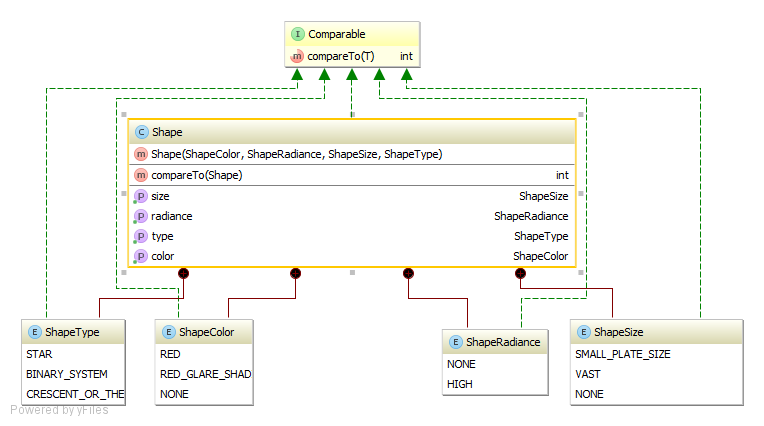
\includegraphics[scale=0.6]{./img/Shape.png}
            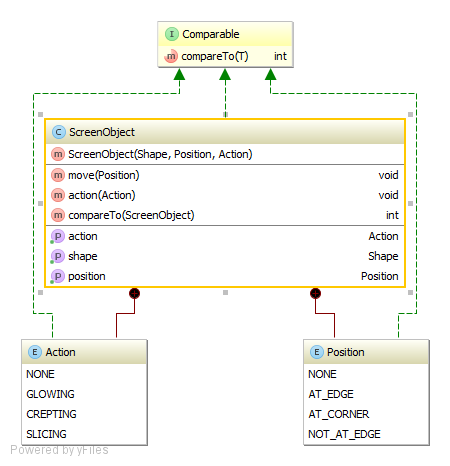
\includegraphics[scale=0.6]{./img/ScreenObject.png}
            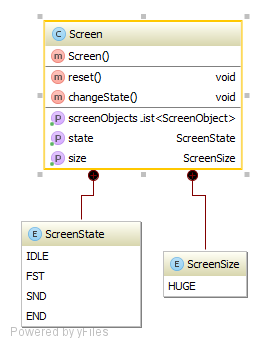
\includegraphics[scale=0.6]{./img/Screen.png}
            \caption{UML диаграмма доменной модели}
        \end{figure}     
\newpage
\section*{Вывод}
    В ходе выполнения лабораторных работ было проведено тестирование разработанных программных модулей.
    При выполнении работы использовались библиотеки JUnit4 и JUnit5. Явных отличий этих библиотек
    в данной работе отмеченно не было, разве что JUnit5 имеет иную иерахию классов и модульность, 
    что делает его более гибким в сравнении с JUnit4, в котором все модули включены в платформу.
\end{document}
